\chapter{Arhitektura i dizajn sustava}

		
		\textbf{\textit{dio 1. revizije}}\\

		\textit{ Potrebno je opisati stil arhitekture te identificirati: podsustave, preslikavanje na radnu platformu, spremišta podataka, mrežne protokole, globalni upravljački tok i sklopovsko-programske zahtjeve. Po točkama razraditi i popratiti odgovarajućim skicama:}
	\begin{itemize}
		\item 	\textit{izbor arhitekture temeljem principa oblikovanja pokazanih na predavanjima (objasniti zašto ste baš odabrali takvu arhitekturu)}
		\item 	\textit{organizaciju sustava s najviše razine apstrakcije (npr. klijent-poslužitelj, baza podataka, datotečni sustav, grafičko sučelje)}
		\item 	\textit{organizaciju aplikacije (npr. slojevi frontend i backend, MVC arhitektura) }		
	\end{itemize}

	
		

		

				
		\section{Baza podataka}
			
			
		Za potrebe našeg sustava koristit ćemo SQL relacijsku bazu podataka. Relacijska baza podataka najviše nam odgovara zbog olakšanog modeliranja događaja i entiteta iz stvarnog svijeta. Osnovna jedinka baze podataka je relacija, to jest tablica koja ima svoj naziv i potreban skup atributa. Zadaća baze podataka je brza i jednostavna pohrana, izmjena i dohvat podataka koje potom treba obraditi. Sve su relacije u bazi svedene na treću normalnu formu kako baza ne bi sadržavala redundantne podatke. Prilikom izrade baze podataka poslužili smo se PostgreSQL-om.
		Baza podataka ove aplikacije sastoji se od sljedećih entiteta:
		\begin{itemize}
			\item 	Profil
			\item 	KorisničkiRačun
			\item   TipUloge
			\item   Kredit
			\item   Transakcija
			\item   Račun
			\item   Vrsta računa
			\item   Kartica
			\item   VrstaKartice		
		\end{itemize}
		
			\subsection{Opis tablica}
			

				\textbf{Profil} Ovaj entitet sadrži sve važne informacije za pristup web aplikaciji. Sadrži atribute: ime, prezime, OIB, adresa prebivališta, datum rođenja, e-mail adresa i slika profila. Ovaj entitet u vezi je \textit{Zero-to-Many} s entitetom Korisnički račun preko OIB-a.  
				
				\begin{longtabu} to \textwidth {|X[6, l]|X[6, l]|X[20, l]|}
					
					\hline \multicolumn{3}{|c|}{\textbf{Profil }}	 \\[3pt] \hline
					\endfirsthead
					
					\hline \multicolumn{3}{|c|}{\textbf{Profil}}	 \\[3pt] \hline
					\endhead
					
					\hline 
					\endlastfoot
					
					Ime & VARCHAR	&  	ime korisnika\cellcolor{LightGreen} 	\\ \hline
					Prezime	& VARCHAR &  prezime korisnika 	\\ \hline 
					\rowcolor{lightgreen}OIB & INT &  OIB korisnika \\ \hline 
					Adresa prebivališta & VARCHAR &   adresa korisnika      \\ \hline
					Datum rođenja & DATE & datum rođenja korisnika \\ \hline
					Email & VARCHAR & e-mail adresa korisnika \\ \hline
					Slika & LONGBLOB & slika korisnika \\ \hline
					
					 
					
					
				\end{longtabu}
			
			\textbf{Korisnički Račun}  Ovaj entitet sadrži sve važne informacije o korisničkom računu. Sadrži atribute: OIB, korisničko ime, lozinka i razina ovlasti. Ovaj entitet je u vezi \textit{Many-to-Zero} sa entitetom Profil preko OIB-a i sa entitetom Tip Uloge \textit{{One-to-One}} preko razine ovlasti. 
			
			\begin{longtabu} to \textwidth {|X[6, l]|X[6, l]|X[20, l]|}
				
				\hline \multicolumn{3}{|c|}{\textbf{Korisnički račun }}	 \\[3pt] \hline
				\endfirsthead
				
				\hline \multicolumn{3}{|c|}{\textbf{Korisnički račun}}	 \\[3pt] \hline
				\endhead
				
				\hline 
				\endlastfoot
				
				\cellcolor{LightGreen}Korisničko ime & VARCHAR	&  jedinstveni identifikator korisnika \\ \hline
				Lozinka	& VARCHAR &   hash lozinke	\\ \hline 
				OIB & INT & OIB korisnika (profil.OIB)\\ \hline
				Razina ovlasti & INT & broj tipa uloge (tipUloge.brojUloge)\\ \hline
				
			\end{longtabu}
		

	
		
			
		\textbf{Tip uloge}  Ovaj entitet sadrži informacije vezane za tipove uloge. Sadrži atribute: broj tipa uloge i naziv uloge. Ovaj je entitet u vezi \textit{One-to-One} s entitetom Korisnički račun preko broja uloge.  
		
		\begin{longtabu} to \textwidth {|X[6, l]|X[6, l]|X[20, l]|}
			
			\hline \multicolumn{3}{|c|}{\textbf{Tip uloge}}	 \\[3pt] \hline
			\endfirsthead
			
			\hline \multicolumn{3}{|c|}{\textbf{Tip uloge}}	 \\[3pt] \hline
			\endhead
			
			\hline 
			\endlastfoot
			
		    Broj uloge & INT & Broj tipa uloge  \\ \hline
			\cellcolor{LightGreen}Naziv & VARCHAR	& Naziv uloge	\\ \hline
			
			
			
			
			
		\end{longtabu}
	
		
		
			\textbf{Kredit}   Ovaj entitet sadrži sve važne informacije o kreditu koji klijent zatraži. Sadrži atribute: broj kredita, OIB, iznos, vrsta kredita, datum ugovaranja, vremenski period otplate kredita i datum rate. U vezi je \textit{One-to-One} s entitetom Vrsta Kredita preko vrste kredita i u vezi \textit{Many-to-One} s entitetom Profil preko OIB-a.
		
		\begin{longtabu} to \textwidth {|X[6, l]|X[6, l]|X[20, l]|}
			
			\hline \multicolumn{3}{|c|}{\textbf{Kredit}}	 \\[3pt] \hline
			\endfirsthead
			
			\hline \multicolumn{3}{|c|}{\textbf{Kredit}}	 \\[3pt] \hline
			\endhead
			
			\hline 
			\endlastfoot
			
			Broj kredita & LONG & broj kredita \\ \hline
			OIB & INT & OIB korisnika (profil.OIB)\\ \hline
			Iznos & DECIMAL (10, 2) & iznos kredita \\ \hline
			Vrsta & VARCHAR & vrsta kredita (vrstaKredita.tipKredita) \\ \hline
			Datum ugovaranja & DATE & datum ugovaranja kredita \\ \hline
			Vremenski period otplate & INT & duljina otplate kredita \\ \hline
			Datum rate & DATE & datum plaćanja mjesečne rate \\ \hline
			
			
			
			
		\end{longtabu}
	
			\textbf{Vrsta kredita} Ovaj entitet sadrži sve važne informacije o vrsti kredita. Sadrži atribute: tip kredita, naziv vrste kredita i kamatnu stopu. U vezi je \textit{One-to-One} sa entitetom Kredit preko tipa kredita. 
	
		\begin{longtabu} to \textwidth {|X[6, l]|X[6, l]|X[20, l]|}
		
			\hline \multicolumn{3}{|c|}{\textbf{Vrsta kredita}}	 \\[3pt] \hline
			\endfirsthead
		
			\hline \multicolumn{3}{|c|}{\textbf{Vrsta kredita}}	 \\[3pt] \hline
			\endhead
		
			\hline 
			\endlastfoot
			
			Tip kredita & INT & broj vrste kredita\\ \hline
			Naziv vrste kredita & VARCHAR & vrsta kredita\\ \hline
			Kamatna stopa & DECIMAL (2,2) &iznos kamatne stope\\ \hline
			
		
		
		
		
		\end{longtabu}
	
		
				\textbf{Transakcija}   Ovaj entitet sadrži sve važne informacije o transakcijama koje klijent želi provesti. Sadrži atribute: broj transakcije, broj računa terećenja, račun odobrenja, datum transakcije i iznos . Entitet Transakcija u vezi je \textit{Many-to-One} s entitetom Račun preko broja računa terećenja i broja računa odobrenja.
			
			\begin{longtabu} to \textwidth {|X[6, l]|X[6, l]|X[20, l]|}
				
				\hline \multicolumn{3}{|c|}{\textbf{Transakcija}}	 \\[3pt] \hline
				\endfirsthead
				
				\hline \multicolumn{3}{|c|}{\textbf{Transakcija}}	 \\[3pt] \hline
				\endhead
				
				\hline 
				\endlastfoot
				
				Broj transakcije & INT & broj transakcije \\ \hline
				Račun terećenja & INT & broj računa terećenja (račun.brojRačuna) \\ \hline
				Račun odobrenja & INT & broj računa odobrenja (račun.brojRačuna) \\ \hline
				Datum transakcije & DATE & datum transakcije \\ \hline
				Iznos & DECIMAL (10, 2) & iznos uplate \\ \hline
				
				
				
				
				
				
				
			\end{longtabu}
		
			\textbf{Račun}   Ovaj entitet sadrži sve važne informacije o računu koji ima klijent. Sadrži atribute: broj računa, OIB klijenta, datum otvaranja računa, stanje računa, vrsta računa, broj kartice, prekoračenje, kamatna stopa i datum zatvaranja. U vezi je  \textit{Many-to-One} s entitetom Profil preko OIB-a, sa entitetom Vrsta Računa \textit{One-to-One} preko vrste računa. Također je u vezi \textit{One-to-Many} s entitetom Transakcija preko broja računa i u vezi je \textit{One-to-Many} s entitetom Kartica preko broja kartice.
		
		\begin{longtabu} to \textwidth {|X[6, l]|X[6, l]|X[20, l]|}
			
			\hline \multicolumn{3}{|c|}{\textbf{Račun}}	 \\[3pt] \hline
			\endfirsthead
			
			\hline \multicolumn{3}{|c|}{\textbf{Račun}}	 \\[3pt] \hline
			\endhead
			
			\hline 
			\endlastfoot
			
			Broj računa & VARCHAR & broj računa \\ \hline
			OIB & INT & OIB korisnika (profil.OIB) \\ \hline
			Datum otvaranja & DATE & datum otvaranja računa \\ \hline
			Stanje & DECIMAL (10, 2) & trenutno stanje računa \\ \hline
			Vrsta računa & INT & broj vrste računa (vrstaRačuna.vrstaRačuna) \\ \hline
			Broj kartice & LONG & broj kartice vezane uz račun (kartica.brojKartice)\\ \hline
			Prekoračenje & DECIMAL(10,2) & iznos prekoračenja računa \\ \hline
			Kamatna stopa & DECIMAL(2, 2) & iznos kamatne stope \\ \hline
			Datum zatvaranja & DATE & datum zatvaranja računa \\ \hline
			
			
			
			
			
			
		\end{longtabu}
	
				\textbf{Vrsta računa}   Ovaj entitet sadrži sve važne informacije o vrsti računa koje neki klijent posjeduje. Sadrži atribute: broj vrste računa i naziv računa. U vezi je \textit{One-to-One} s entitetom Račun preko vrste računa.
			\begin{longtabu} to \textwidth {|X[6, l]|X[6, l]|X[20, l]|}
				
				\hline \multicolumn{3}{|c|}{\textbf{Vrsta računa}}	 \\[3pt] \hline
				\endfirsthead
				
				\hline \multicolumn{3}{|c|}{\textbf{Vrsta računa}}	 \\[3pt] \hline
				\endhead
				
				\hline 
				\endlastfoot
				
				Vrsta računa & INT & Broj vrste računa \\ \hline
				Naziv računa & VARCHAR & Naziv vrste računa \\ \hline
				
				
				
				
	\end{longtabu}	
		
		
			\textbf{Kartica}   Ovaj entitet sadrži sve važne informacije o karticama koje ima klijent. Sadrži atribute: broj kartice, OIB, broj tipa kartice, stanje, valjanost,limit, kamatna stopa i datum rate. U vezi je \textit{Many-to-One} s entitetom Račun preko broja kartice i sa entitetom Vrsta kartice \textit{One-to-One} preko tipa kartice. 
			
			\begin{longtabu} to \textwidth {|X[6, l]|X[6, l]|X[20, l]|}
				
				\hline \multicolumn{3}{|c|}{\textbf{Kartica}}	 \\[3pt] \hline
				\endfirsthead
				
				\hline \multicolumn{3}{|c|}{\textbf{Kartica}}	 \\[3pt] \hline
				\endhead
				
				\hline 
				\endlastfoot
				
				Broj kartice & INT & broj kartice\\ \hline
				OIB & INT & OIB klijenta (profil.OIB)\\ \hline
				Tip kartice & INT & broj tipa kartice (vrstaKartice.tipKartice)\\ \hline
				Stanje & DECIMAL(10,2) & stanje kartice\\ \hline
				Valjanost & DATE & datum isteka valjanosti kartice \\ \hline
				Limit & DECIMAL (10,2)& odobren limit \\ \hline
				Kamatna stopa & DECIMAL(2, 2) & iznos kamatne stope \\ \hline
				Datum rate & DATE & datum otplate dugovanja kartice \\ \hline
	
		

		\end{longtabu}	
	
			\textbf{Vrsta kartice}   Ovaj entitet sadrži sve važne informacije o vrstama kartice koje ima klijent. Sadrži atribute:broj tipa kartice i naziv kartice. U vezi je \textit{One-to-One} s entitetom Kartica preko tipa kartice.
			\begin{longtabu} to \textwidth {|X[6, l]|X[6, l]|X[20, l]|}
				
				\hline \multicolumn{3}{|c|}{\textbf{Vrsta kartice}}	 \\[3pt] \hline
				\endfirsthead
				
				\hline \multicolumn{3}{|c|}{\textbf{Vrsta kartice}}	 \\[3pt] \hline
				\endhead
				
				\hline 
				\endlastfoot
		
				Tip kartice & INT & broj tipa kartice\\ \hline
				Naziv kartice & VARCHAR & naziv kartice\\ \hline
		
		
		
		\end{longtabu}
	
				
		
		
		
			
			\subsection{Dijagram baze podataka}
				\begin{figure}[H]
					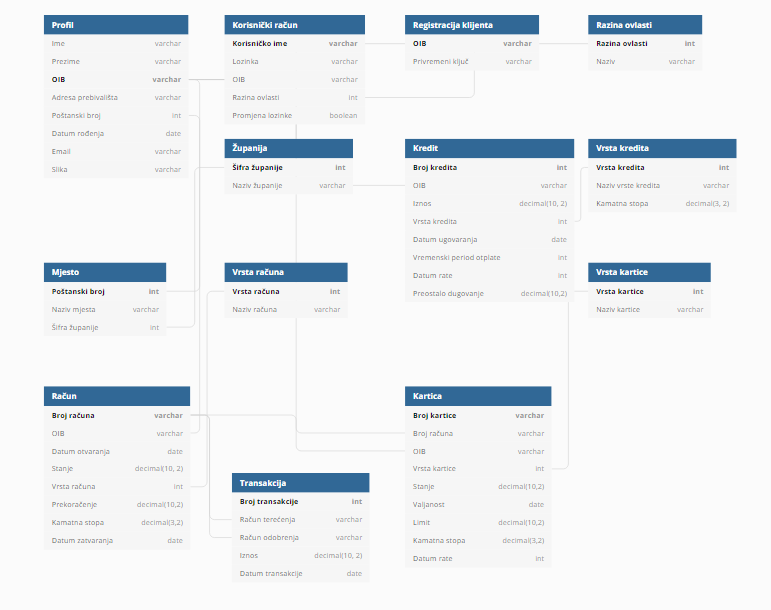
\includegraphics[scale=0.75]{Slike/ermodel.PNG}
					\centering
					\caption{E-R dijagram baze podataka}
					\label{fig:dijagram}
				\end{figure}
			\eject
			
			
		\section{Dijagram razreda}
		
			\textit{Potrebno je priložiti dijagram razreda s pripadajućim opisom. Zbog preglednosti je moguće dijagram razlomiti na više njih, ali moraju biti grupirani prema sličnim razinama apstrakcije i srodnim funkcionalnostima.}\\
			
			\textbf{\textit{dio 1. revizije}}\\
			
			\textit{Prilikom prve predaje projekta, potrebno je priložiti potpuno razrađen dijagram razreda vezan uz \textbf{generičku funkcionalnost} sustava. Ostale funkcionalnosti trebaju biti idejno razrađene u dijagramu sa sljedećim komponentama: nazivi razreda, nazivi metoda i vrste pristupa metodama (npr. javni, zaštićeni), nazivi atributa razreda, veze i odnosi između razreda.}\\
			
			\textbf{\textit{dio 2. revizije}}\\			
			
			\textit{Prilikom druge predaje projekta dijagram razreda i opisi moraju odgovarati stvarnom stanju implementacije}
			
			
			
			\eject
		
		\section{Dijagram stanja}
			
			
			\textbf{\textit{dio 2. revizije}}\\
			
			\textit{Potrebno je priložiti dijagram stanja i opisati ga. Dovoljan je jedan dijagram stanja koji prikazuje \textbf{značajan dio funkcionalnosti} sustava. Na primjer, stanja korisničkog sučelja i tijek korištenja neke ključne funkcionalnosti jesu značajan dio sustava, a registracija i prijava nisu. }
			
			
			\eject 
		
		\section{Dijagram aktivnosti}
			
			\textbf{\textit{dio 2. revizije}}\\
			
			 \textit{Potrebno je priložiti dijagram aktivnosti s pripadajućim opisom. Dijagram aktivnosti treba prikazivati značajan dio sustava.}
			
			\eject
		\section{Dijagram komponenti}
		
			\textbf{\textit{dio 2. revizije}}\\
		
			 \textit{Potrebno je priložiti dijagram komponenti s pripadajućim opisom. Dijagram komponenti treba prikazivati strukturu cijele aplikacije.}